\documentclass[../Main.tex]{subfiles} 
\begin{document}

\section{Algorithms}
% \subsection{Main algorithm}
% \subsection{Difference between both attempts}
\subsection{Cosine similarity}
\begin{figure}
  \[ sim(\vec{q},\vec{d_j}) = \frac{\sum^N_{i=1} w_{i,q} \times w_{i,j}}{\sqrt{\sum^N_{i=1}w^2_{i,q}} \times \sqrt{\sum^N_{i=1}w^2_{i,j}}} \]
  \caption{Cosine similarity}
  \label{cos_sim}
\end{figure}
\begin{figure}
 \begin{align*}
  q &= \textrm{'Ich glaube @Drahflow tippt noch schneller als er redet. ;) \#om13' } \\
  \vec{q} &= (0.427, 0.38, 0.4, 0.39, 0.391, 0.602,  0.41) \\ 
   \vec{\bar{d}} &= \frac{\sum^N_{i=0} d_i}{N} =  (0.376, 0.336, 0.349, 0.346, 0.361, 0.481,  0.379) \\
  sim(\vec{q}, \vec{\bar{d}}) &= 0.9986 
\end{align*}
  \caption{Example for the similarity calculation}
  \label{cos_sim_example}
\end{figure}
Although Tweets may differ from one region to another in some way, a huge percentage of the German Twitter users write their messages exclusively in standard German with no signs of any regional influence whatsoever.  \\
For example the following Tweet just appeared in my timeline:
\begin{quote}
'Ich glaube @Drahflow tippt noch schneller als er redet. ;) \#om13'
\end{quote}
Keeping in mind that  usernames, hashtags, smileys and punctation are being removed in the pre-processing, this Tweet contains way to ordinary words to be assigned to a specific region. It is written in pure High German and therefore could be sent from a town in Bavaria as well as from Berlin and depending on the data we use to train our algorithm with, the result of the program could be 'Austria' or 'Northern Germany' as well.

To face this problem we decided to filter this kind of undistinguished Tweets to have more reliable results and because of that also increase the accuracy of the algorithm. \\
Our idea was to determine the average Tweet-vector $\vec{\bar{d}}$ of all the Tweets in the training-corpus and to compare the Tweet-vector $\vec{q}$ of a given Tweet with it, using the cosine metric (see Figure \ref{cos_sim} on page \pageref{cos_sim}) as recommended  in Jurafsky \& Martin. If the similarity between both vectors is smaller than a specified threshold, we continue to map the Tweet to one of the region, if not we stop and return a message, that the Tweet is written in standard German and can not be classified. In the example in figure \ref{cos_sim_example} on page \pageref{cos_sim_example}, the vector $\vec{q}$ for the Tweet mentioned above is compared to the average Tweet-vector $\vec{\bar{d}}$, returning a very high similarity of $0.9986$. Nevertheless the algorithm states, that the Tweet was most likely sent from Switzerland. 

But the most difficult thing was to find the right threshold, that separates the too ordinary Tweets from the regional ones. To make a guess which percentage of all Tweets are written in standard German, we calculated the cosine similarity of all Tweets in the training-corpus to the average vector, sorted them and had a look at the distribution (figure \ref{cos_distribution} in page \pageref{cos_distribution}). \\
The result was not surprising: More than 80\% of all Tweets had a similarity of 0.9 or higher. Or, seen from another point of view, only 20\% of all Tweets differ enough from the average vector to calculate reliable results. 

In the experiments in the sections 3 (regional based attempt) and 4 (geo location based) we tested different thresholds to find a good balance between a reliable classification with a high accuracy and the coverage of as many Tweets as possible.

\begin{figure}
  \begin{center}
   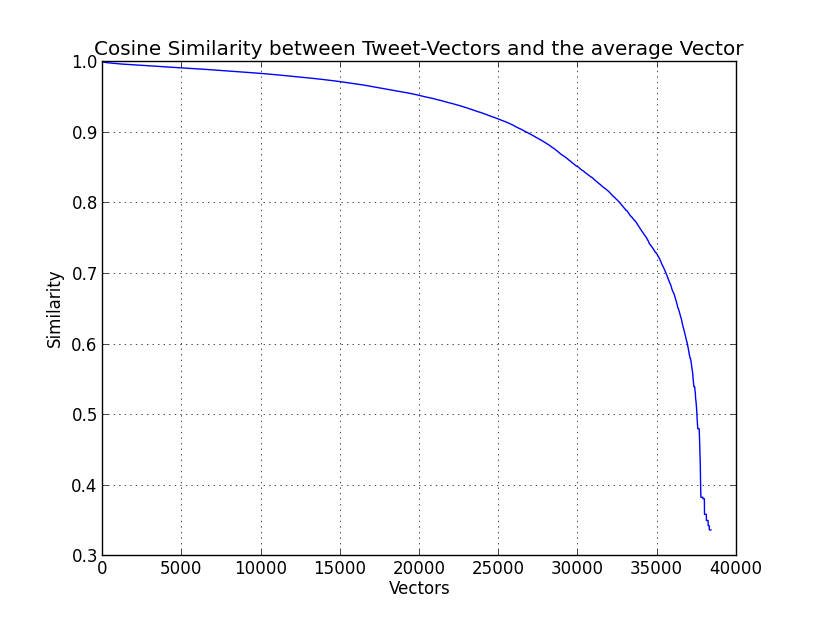
\includegraphics[width=\columnwidth]{img/cos-verteilung.png}
    \caption{\label{cos_distribution} Cosine similarity between all Tweet-vectors and the average Tweet-vector}
  \end{center}
\end{figure}

% \subsection{Evaluation}

\end{document}
